\documentclass{article}
\usepackage[margin=0.4in, letterpaper]{geometry}
\usepackage{hyperref}
\usepackage{graphicx}
\usepackage{float}

\begin{document}
    \graphicspath{ {../plots/} }
    \listoffigures
    \section*{0000}
      \subsection*{test}
                        \begin{figure}[H]
                            \centering
                            \caption{0000 plot of c1 variables using cut: ``test"}
                            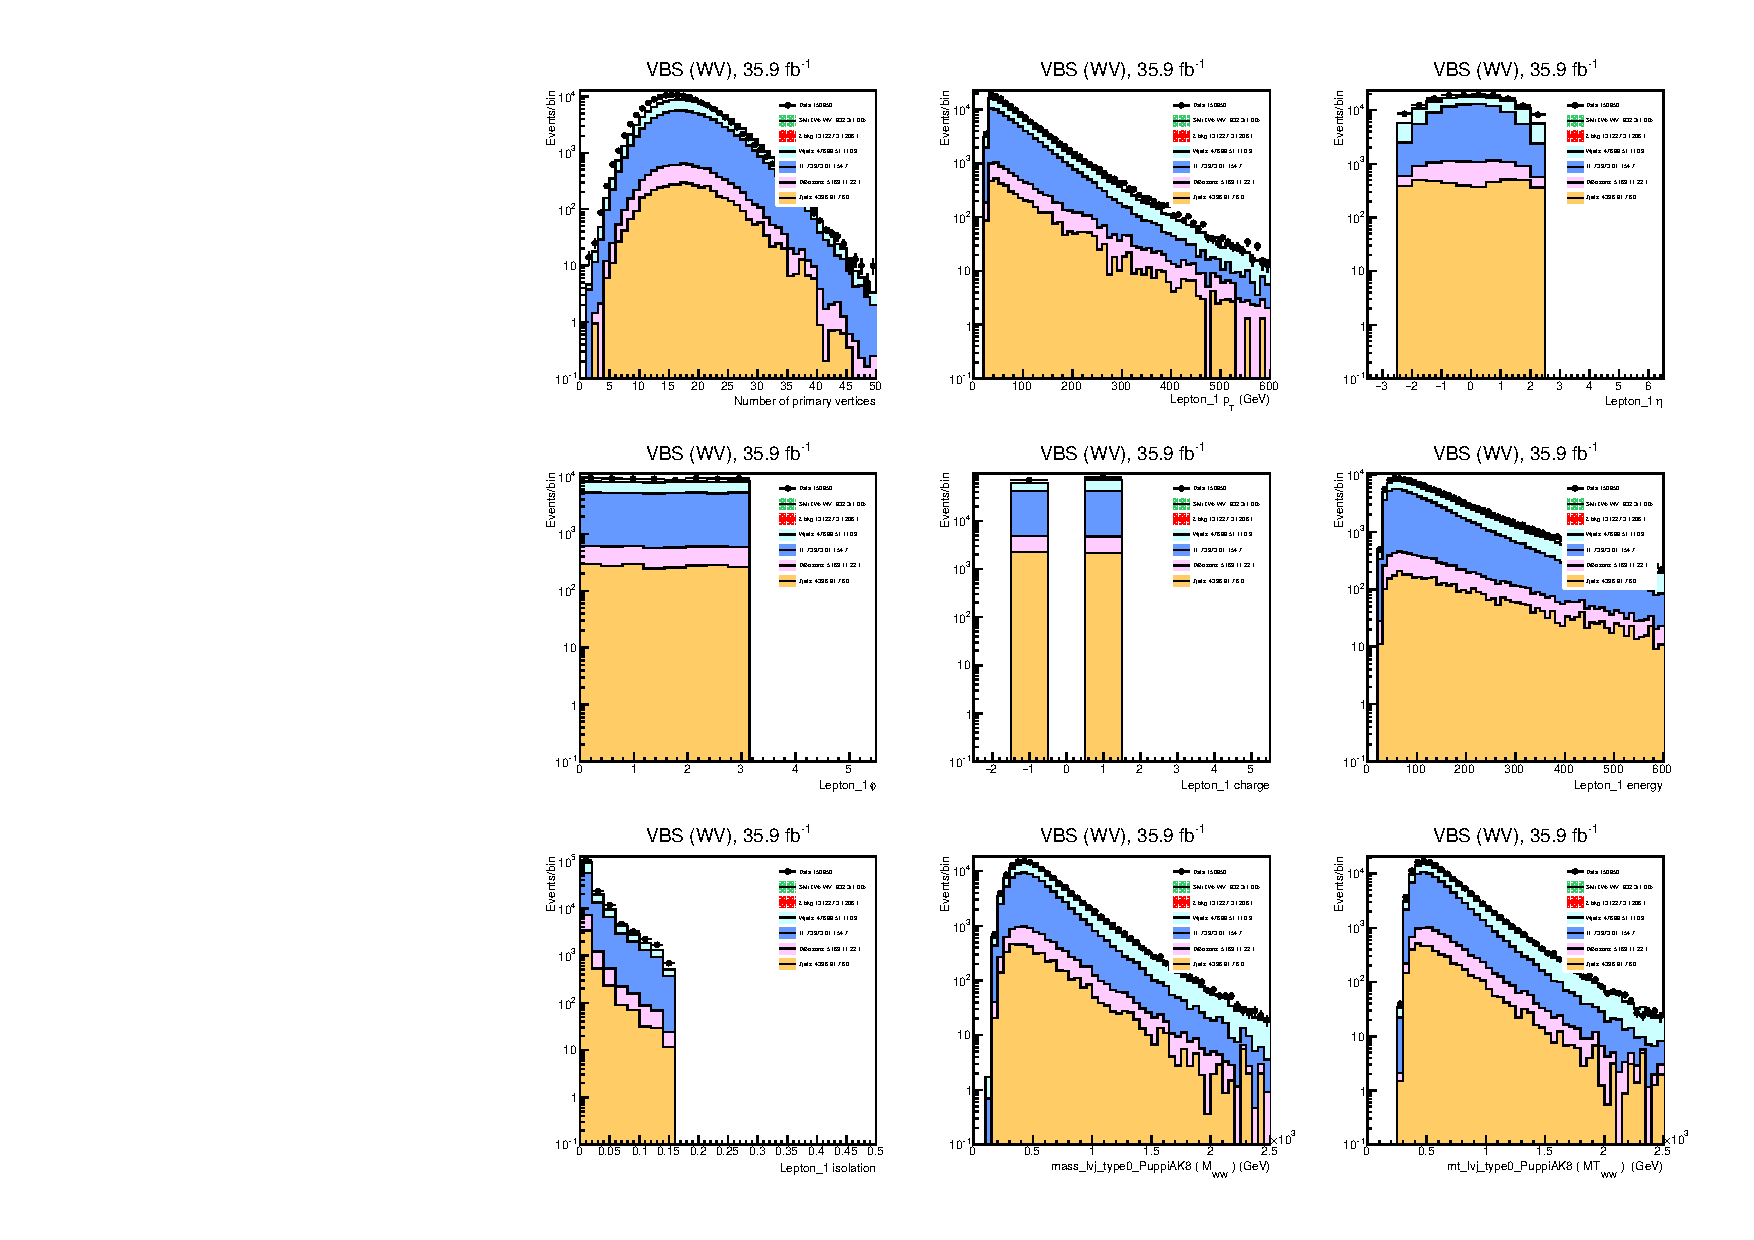
\includegraphics[width=\textwidth]{0000/c1_0000_test.pdf}
                        \end{figure}    
                        \begin{figure}[H]
                            \centering
                            \caption{0000 plot of c2 variables using cut: ``test"}
                            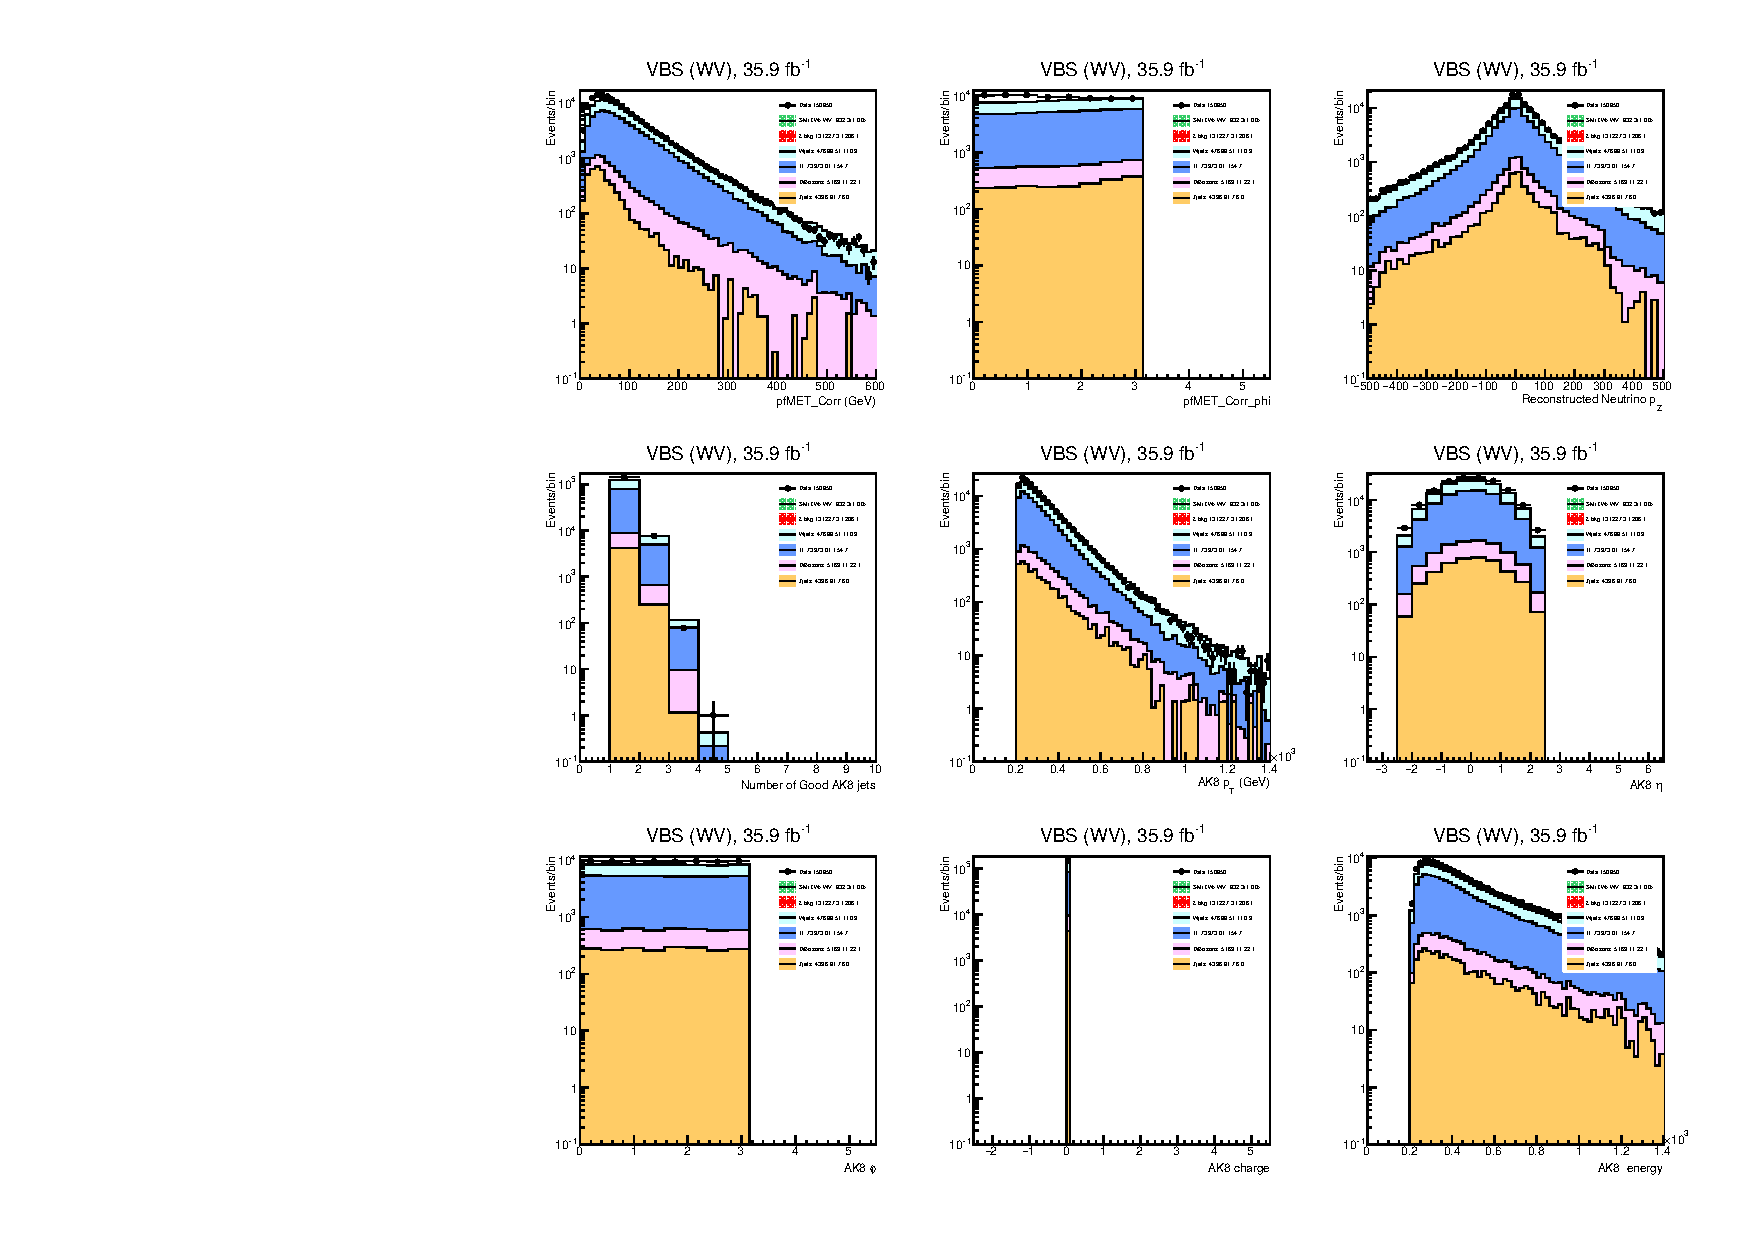
\includegraphics[width=\textwidth]{0000/c2_0000_test.pdf}
                        \end{figure}    
                        \begin{figure}[H]
                            \centering
                            \caption{0000 plot of c3 variables using cut: ``test"}
                            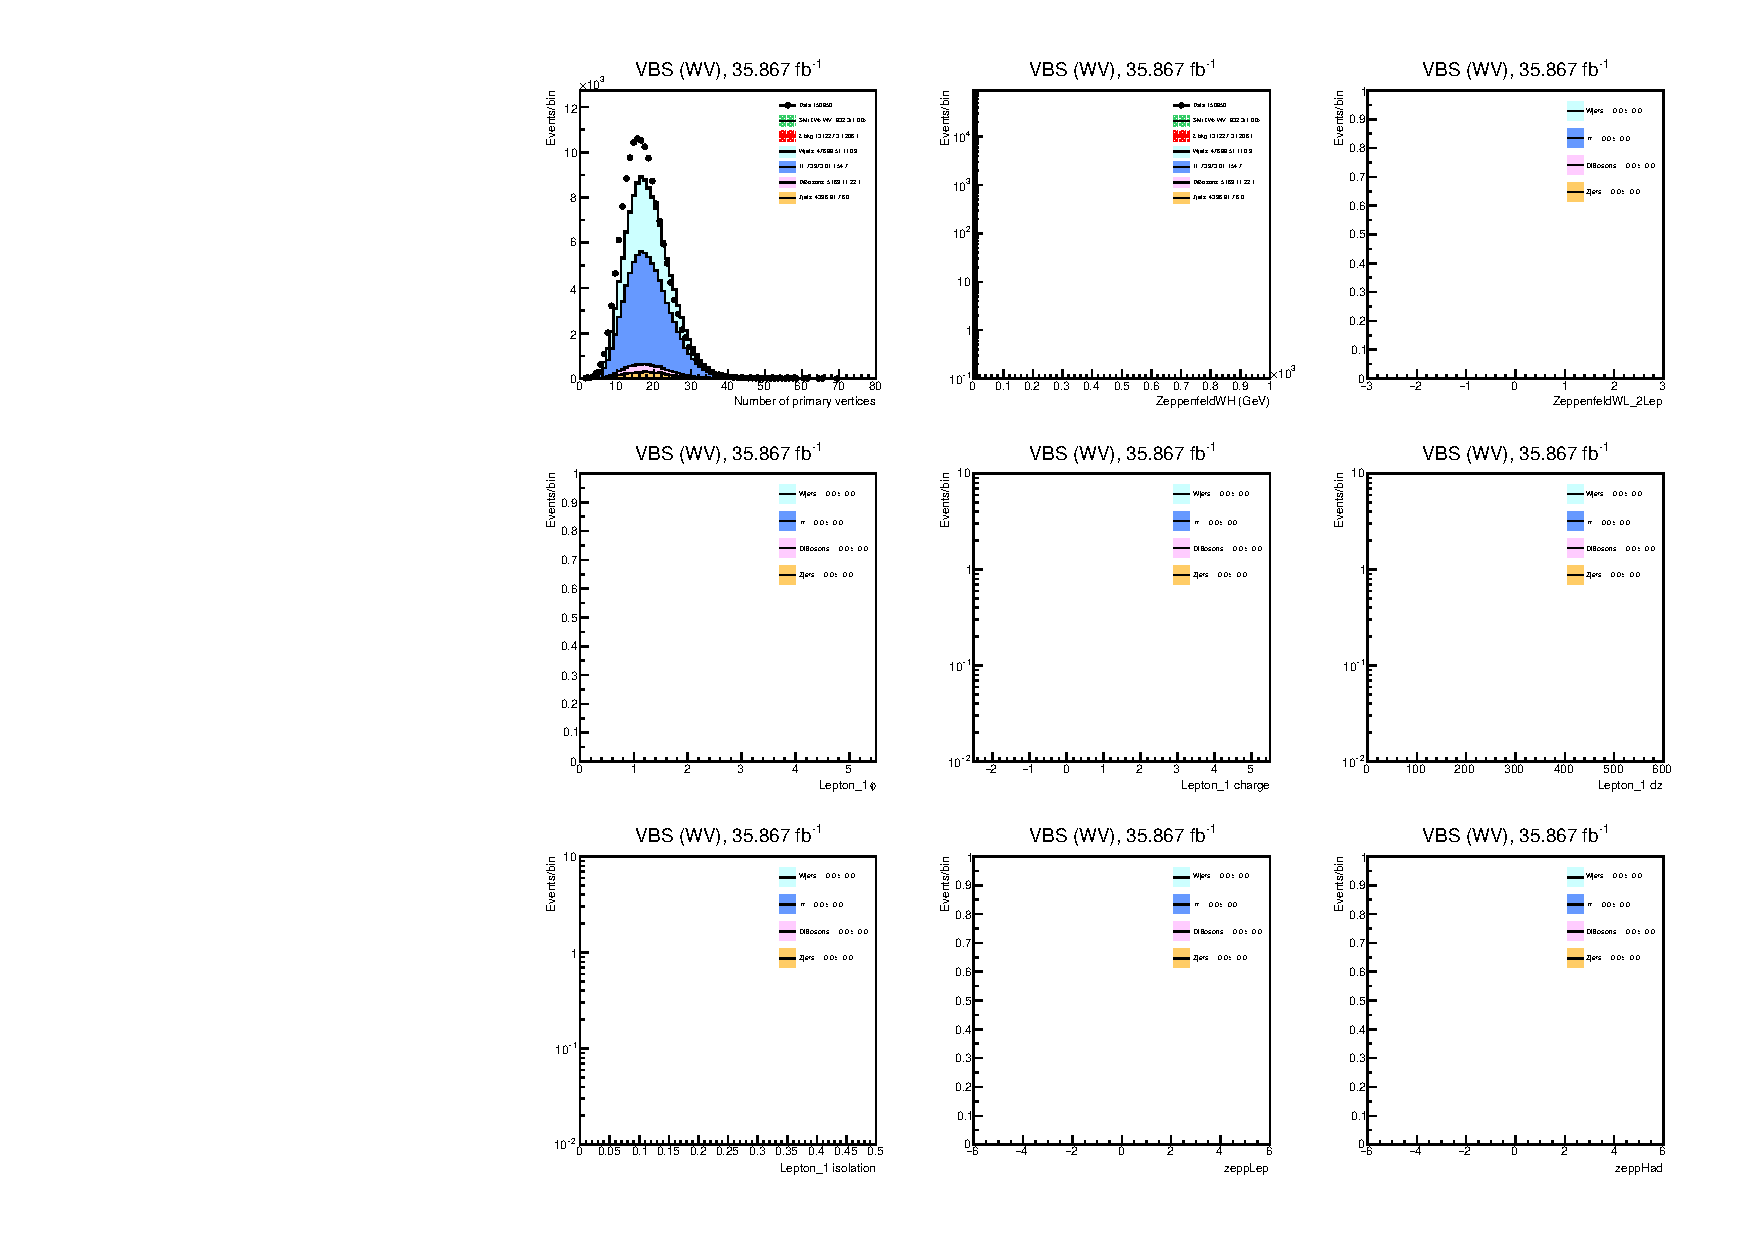
\includegraphics[width=\textwidth]{0000/c3_0000_test.pdf}
                        \end{figure}    
    \section*{2016}
      \subsection*{Full\_SR}
                        \begin{figure}[H]
                            \centering
                            \caption{2016 plot of c1 variables using cut: ``Full\_SR"}
                            \includegraphics[width=\textwidth]{2016/c1_2016_Full_SR.pdf}
                        \end{figure}    
                        \begin{figure}[H]
                            \centering
                            \caption{2016 plot of c2 variables using cut: ``Full\_SR"}
                            \includegraphics[width=\textwidth]{2016/c2_2016_Full_SR.pdf}
                        \end{figure}    
                        \begin{figure}[H]
                            \centering
                            \caption{2016 plot of c3 variables using cut: ``Full\_SR"}
                            \includegraphics[width=\textwidth]{2016/c3_2016_Full_SR.pdf}
                        \end{figure}    
                        \begin{figure}[H]
                            \centering
                            \caption{2016 plot of c4 variables using cut: ``Full\_SR"}
                            \includegraphics[width=\textwidth]{2016/c4_2016_Full_SR.pdf}
                        \end{figure}    
      \subsection*{Top\_CR}
                        \begin{figure}[H]
                            \centering
                            \caption{2016 plot of c1 variables using cut: ``Top\_CR"}
                            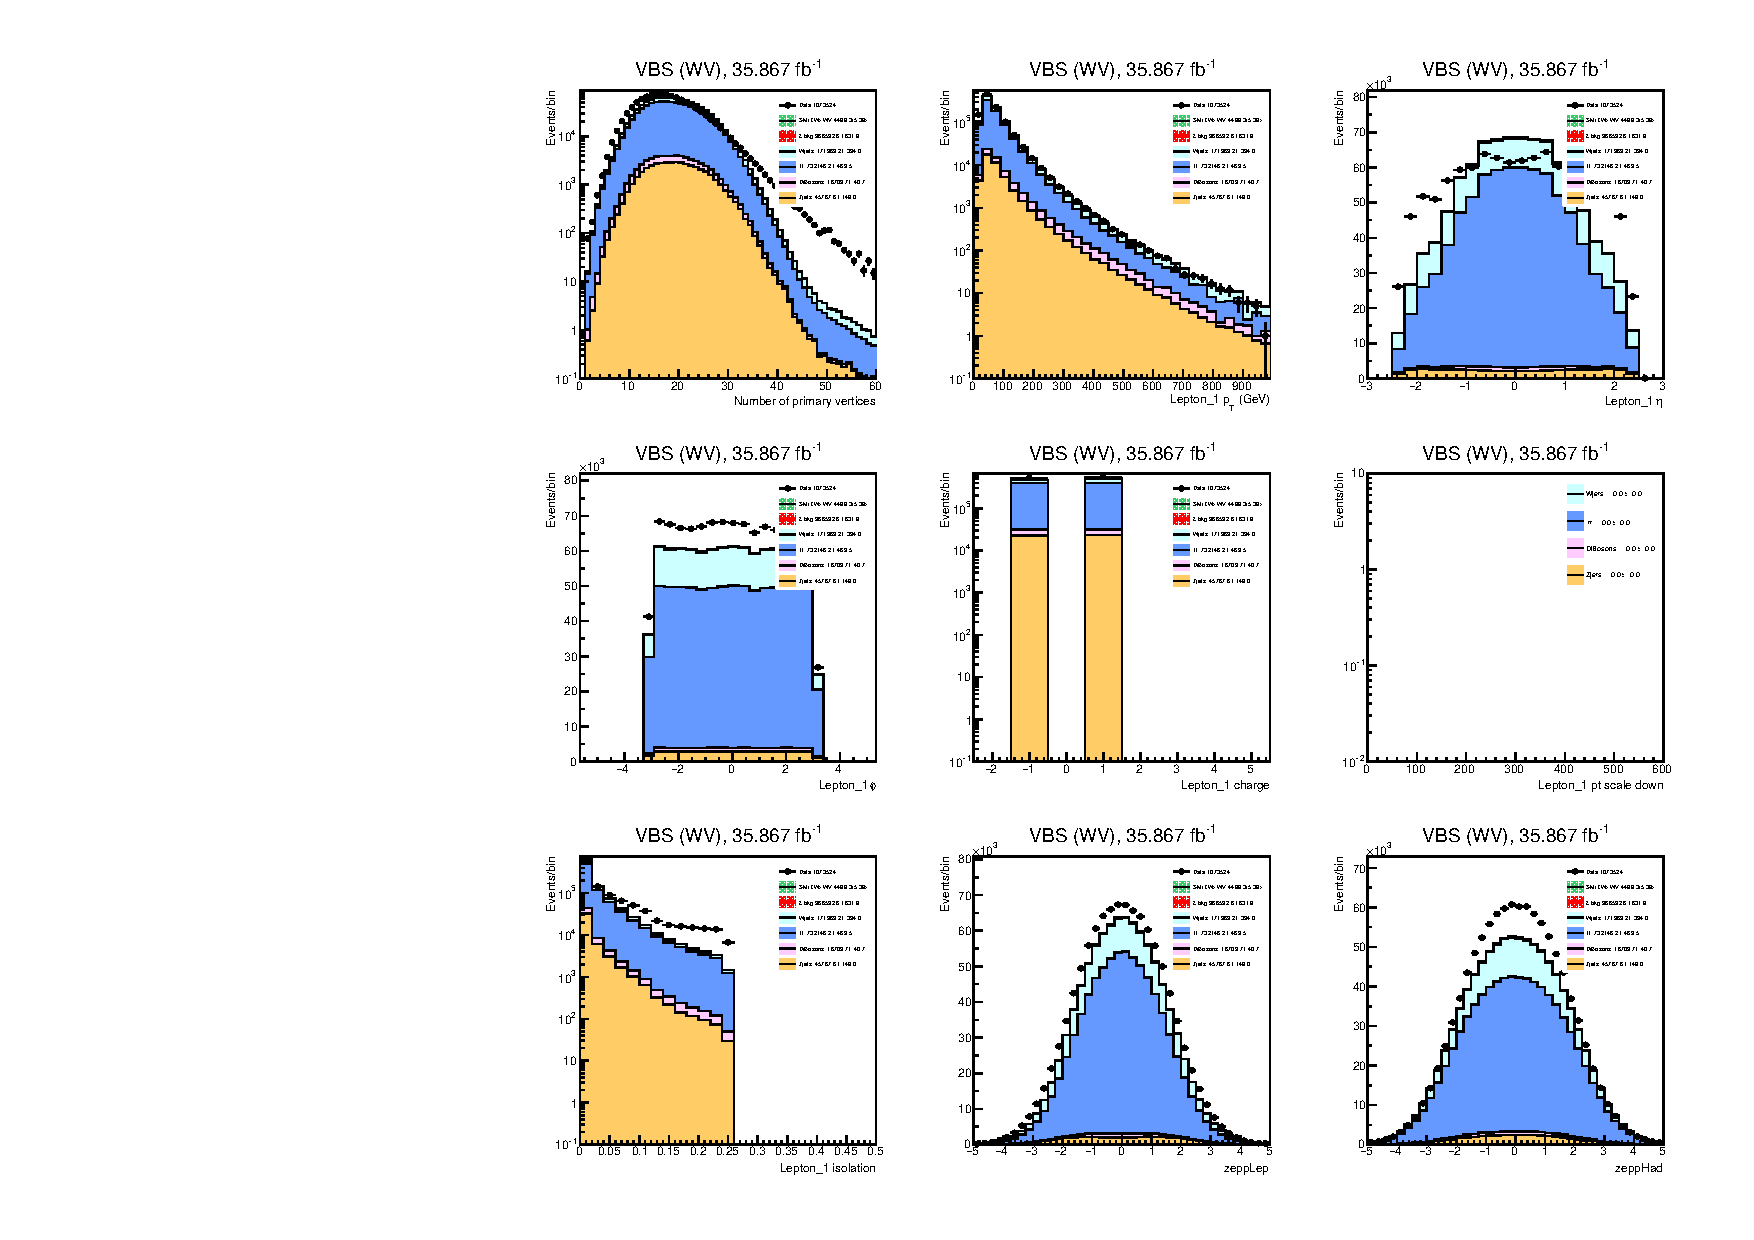
\includegraphics[width=\textwidth]{2016/c1_2016_Top_CR.pdf}
                        \end{figure}    
                        \begin{figure}[H]
                            \centering
                            \caption{2016 plot of c2 variables using cut: ``Top\_CR"}
                            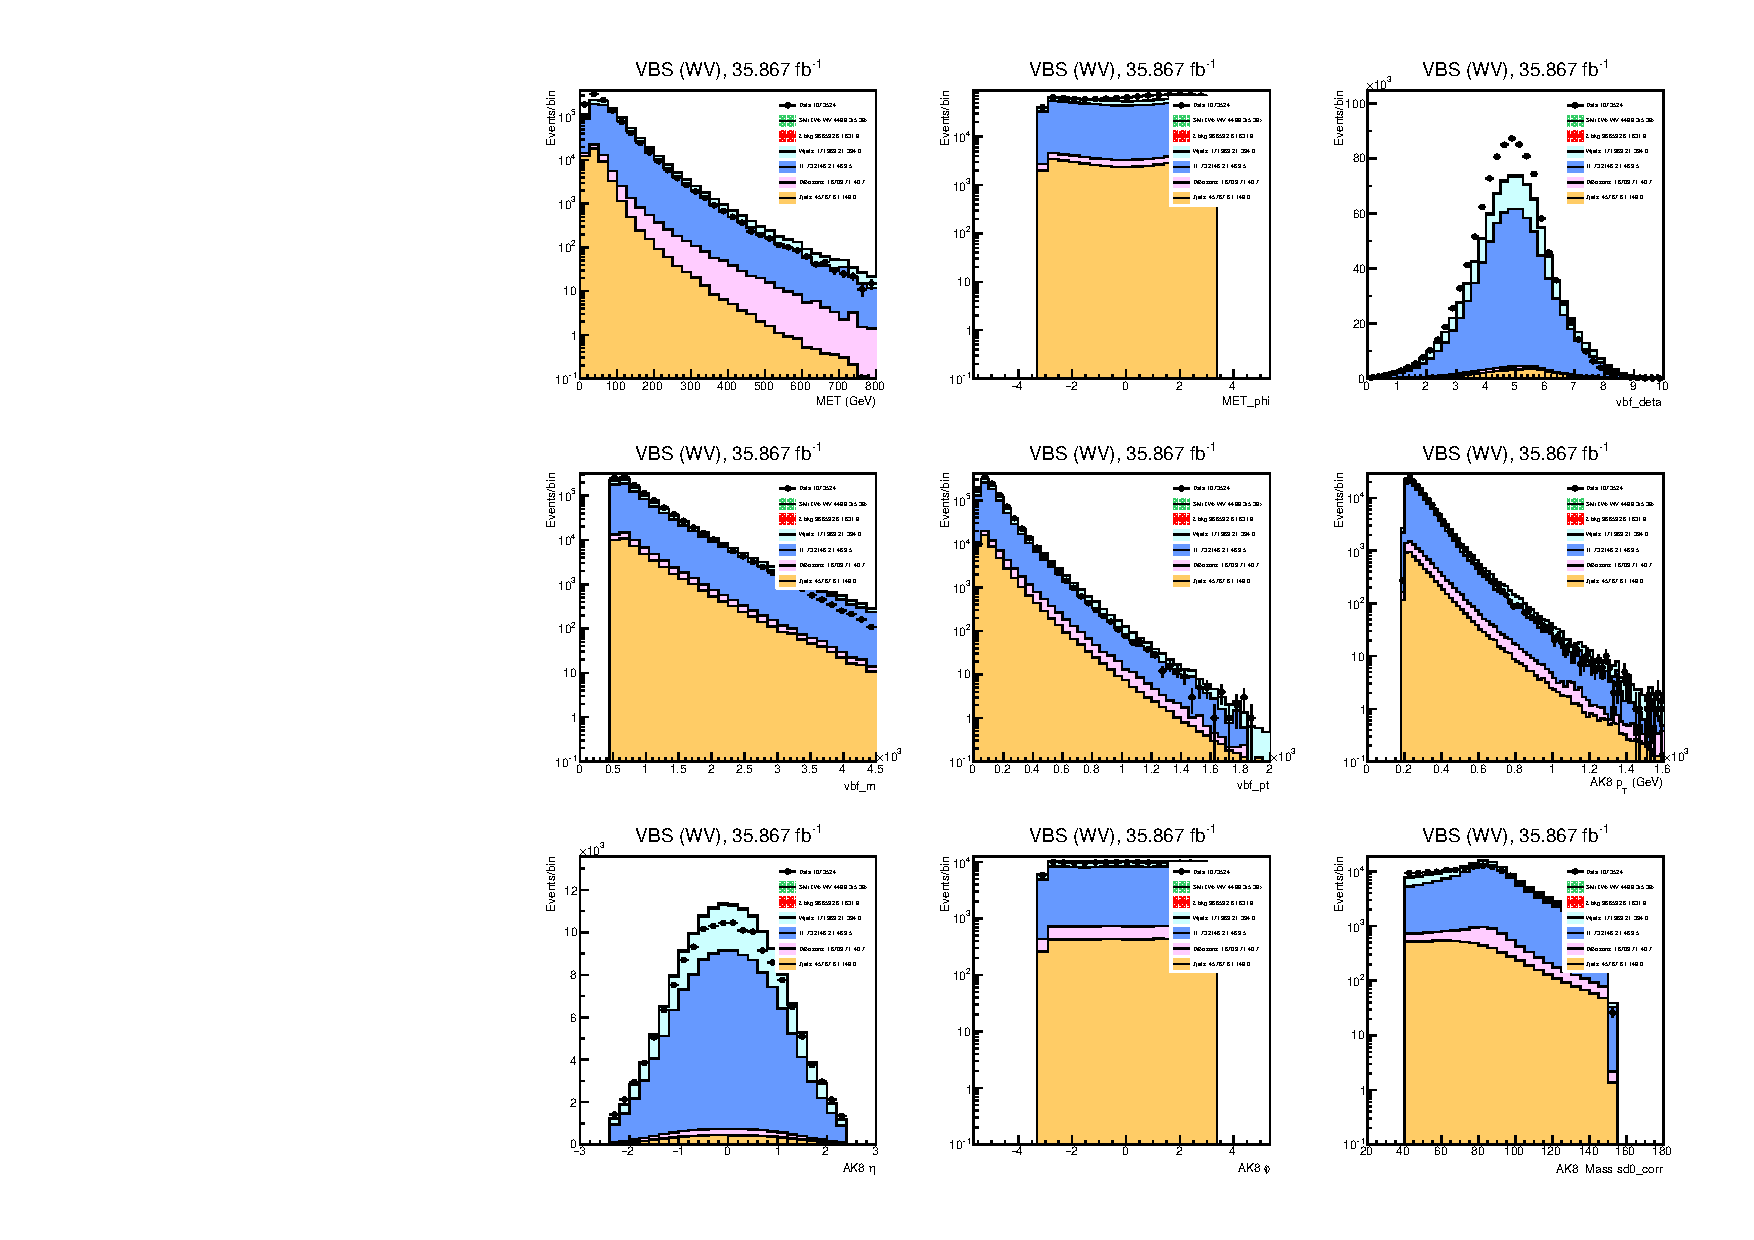
\includegraphics[width=\textwidth]{2016/c2_2016_Top_CR.pdf}
                        \end{figure}    
                        \begin{figure}[H]
                            \centering
                            \caption{2016 plot of c3 variables using cut: ``Top\_CR"}
                            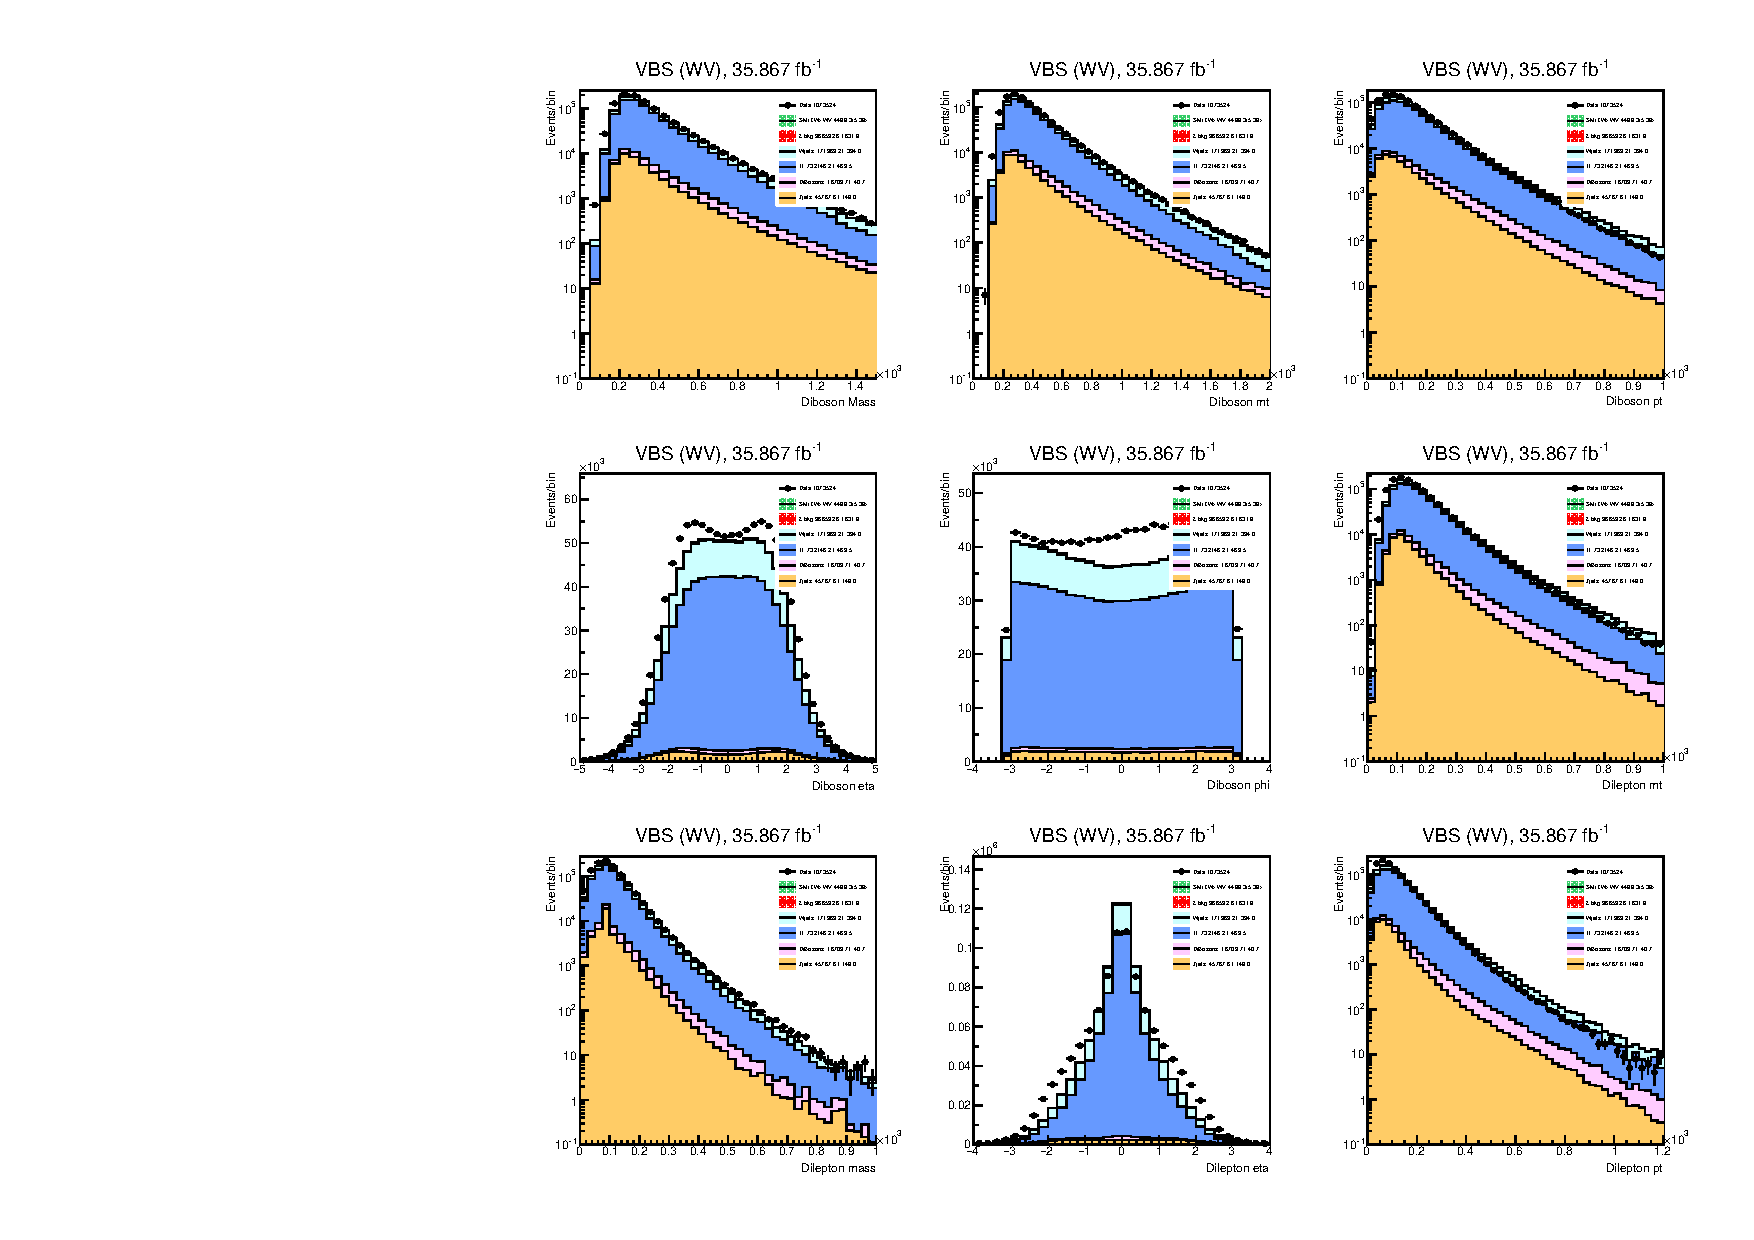
\includegraphics[width=\textwidth]{2016/c3_2016_Top_CR.pdf}
                        \end{figure}    
                        \begin{figure}[H]
                            \centering
                            \caption{2016 plot of c4 variables using cut: ``Top\_CR"}
                            \includegraphics[width=\textwidth]{2016/c4_2016_Top_CR.pdf}
                        \end{figure}    
      \subsection*{Wjets\_CR}
                        \begin{figure}[H]
                            \centering
                            \caption{2016 plot of c1 variables using cut: ``Wjets\_CR"}
                            \includegraphics[width=\textwidth]{2016/c1_2016_Wjets_CR.pdf}
                        \end{figure}    
                        \begin{figure}[H]
                            \centering
                            \caption{2016 plot of c2 variables using cut: ``Wjets\_CR"}
                            \includegraphics[width=\textwidth]{2016/c2_2016_Wjets_CR.pdf}
                        \end{figure}    
                        \begin{figure}[H]
                            \centering
                            \caption{2016 plot of c3 variables using cut: ``Wjets\_CR"}
                            \includegraphics[width=\textwidth]{2016/c3_2016_Wjets_CR.pdf}
                        \end{figure}    
                        \begin{figure}[H]
                            \centering
                            \caption{2016 plot of c4 variables using cut: ``Wjets\_CR"}
                            \includegraphics[width=\textwidth]{2016/c4_2016_Wjets_CR.pdf}
                        \end{figure}    
    \section*{2018}
      \subsection*{Full\_SR}
                        \begin{figure}[H]
                            \centering
                            \caption{2018 plot of c1 variables using cut: ``Full\_SR"}
                            \includegraphics[width=\textwidth]{2018/c1_2018_Full_SR.pdf}
                        \end{figure}    
                        \begin{figure}[H]
                            \centering
                            \caption{2018 plot of c2 variables using cut: ``Full\_SR"}
                            \includegraphics[width=\textwidth]{2018/c2_2018_Full_SR.pdf}
                        \end{figure}    
                        \begin{figure}[H]
                            \centering
                            \caption{2018 plot of c3 variables using cut: ``Full\_SR"}
                            \includegraphics[width=\textwidth]{2018/c3_2018_Full_SR.pdf}
                        \end{figure}    
                        \begin{figure}[H]
                            \centering
                            \caption{2018 plot of c4 variables using cut: ``Full\_SR"}
                            \includegraphics[width=\textwidth]{2018/c4_2018_Full_SR.pdf}
                        \end{figure}    
      \subsection*{Top\_CR}
                        \begin{figure}[H]
                            \centering
                            \caption{2018 plot of c1 variables using cut: ``Top\_CR"}
                            \includegraphics[width=\textwidth]{2018/c1_2018_Top_CR.pdf}
                        \end{figure}    
                        \begin{figure}[H]
                            \centering
                            \caption{2018 plot of c2 variables using cut: ``Top\_CR"}
                            \includegraphics[width=\textwidth]{2018/c2_2018_Top_CR.pdf}
                        \end{figure}    
                        \begin{figure}[H]
                            \centering
                            \caption{2018 plot of c3 variables using cut: ``Top\_CR"}
                            \includegraphics[width=\textwidth]{2018/c3_2018_Top_CR.pdf}
                        \end{figure}    
                        \begin{figure}[H]
                            \centering
                            \caption{2018 plot of c4 variables using cut: ``Top\_CR"}
                            \includegraphics[width=\textwidth]{2018/c4_2018_Top_CR.pdf}
                        \end{figure}    
      \subsection*{Wjets\_CR}
                        \begin{figure}[H]
                            \centering
                            \caption{2018 plot of c1 variables using cut: ``Wjets\_CR"}
                            \includegraphics[width=\textwidth]{2018/c1_2018_Wjets_CR.pdf}
                        \end{figure}    
                        \begin{figure}[H]
                            \centering
                            \caption{2018 plot of c2 variables using cut: ``Wjets\_CR"}
                            \includegraphics[width=\textwidth]{2018/c2_2018_Wjets_CR.pdf}
                        \end{figure}    
                        \begin{figure}[H]
                            \centering
                            \caption{2018 plot of c3 variables using cut: ``Wjets\_CR"}
                            \includegraphics[width=\textwidth]{2018/c3_2018_Wjets_CR.pdf}
                        \end{figure}    
                        \begin{figure}[H]
                            \centering
                            \caption{2018 plot of c4 variables using cut: ``Wjets\_CR"}
                            \includegraphics[width=\textwidth]{2018/c4_2018_Wjets_CR.pdf}
                        \end{figure}    
\end{document}
